% $Id$
%\documentclass[handout]{beamer}
\documentclass{beamer}
\usepackage[utf8]{inputenc}
\usepackage[T1]{fontenc}
\usepackage[english,swedish]{babel}
\usepackage{url}
\usepackage{graphicx}
\usepackage{color}
\usepackage{subfig}
\usepackage{multicol}
\usepackage{csquotes}
\usepackage[natbib,style=alphabetic,maxbibnames=99]{biblatex}
\addbibresource{msbforts.bib}
\setbeamertemplate{bibliography item}[text]

\mode<presentation>{%
  \usetheme{Berlin}
  \setbeamercovered{transparent}
  \setbeamertemplate{footline}{\insertframenumber}
}

\title[Intro infosäk]{%
  Fortsättning av\\
  MSB:s metodstöd
}
\author{Carina Bengtsson och Daniel Bosk\footnote{%
  Detta verk är tillgängliggjort under licensen Creative Commons 
  Erkännande-DelaLika 2.5 Sverige (CC BY-SA 2.5 SE).
	För att se en sammanfattning och kopia av licenstexten besök URL 
	\url{http://creativecommons.org/licenses/by-sa/2.5/se/}.
}}
\institute[MIUN ITM]{%
  Avdelningen för informations- och kommunikationssytem,\\
  Mittuniversitetet, Sundsvall.
}
\date{\today}

\AtBeginSection[]{%
  \begin{frame}<beamer>{Översikt}
    \begin{multicols}{2}
      \tableofcontents[currentsection]
    \end{multicols}
  \end{frame}
}

\begin{document}

\begin{frame}
  \titlepage{}
\end{frame}

\begin{frame}{Översikt}
  \begin{multicols}{2}
    \tableofcontents
  \end{multicols}
	% You might wish to add the option [pausesections]
\end{frame}

% Since this a solution template for a generic talk, very little can
% be said about how it should be structured. However, the talk length
% of between 15min and 45min and the theme suggest that you stick to
% the following rules:  

% - Exactly two or three sections (other than the summary).
% - At *most* three subsections per section.
% - Talk about 30s to 2min per frame. So there should be between about
%   15 and 30 frames, all told.


\section{Analys}

\subsection{Verksamhetsanalys}

\begin{frame}{Vad ska skyddas?}
  \begin{itemize}
    \item Vilka informationstillgångar har vi och hur skyddsvärda är de?
    \item Ska leda till en strukturerad förteckning över
      \begin{itemize}
        \item vilka informationstillgångar som finns,
        \item vilka krav och förväntningar som finns på dessa, samt
        \item vilket värde respektive tillgång har.
      \end{itemize}
  \end{itemize}
\end{frame}

\begin{frame}{Hitta informationstillgångarna}
  \begin{itemize}
    \item Tidigare kartläggningar?
    \item Avdelningsvis?
    \item IT-system?
    \item Projekt?
    \item Processer?
    \item Funktionsvis?
  \end{itemize}
\end{frame}

\begin{frame}{MSB:s förslag på klassificeringsmodell}
  \begin{figure}
    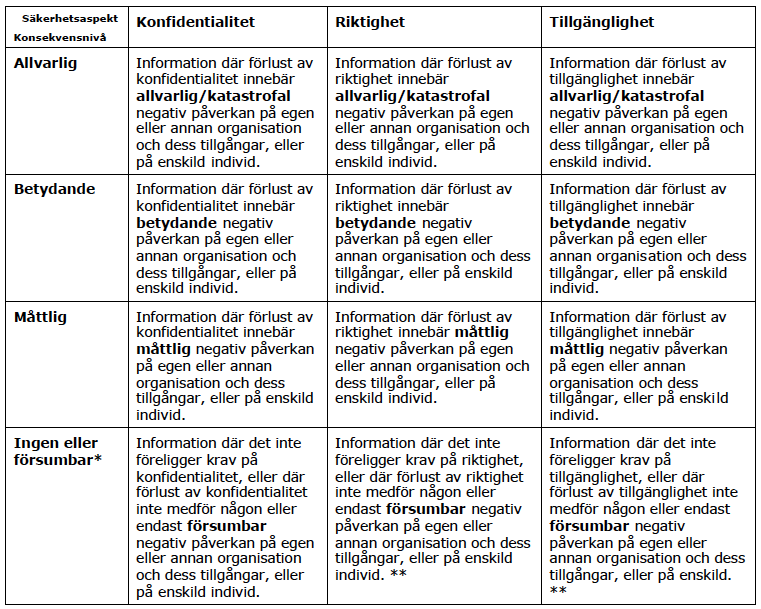
\includegraphics[height=0.7\textheight]{msb-klassificering.png}
    \caption{MSB:s förslag på klassificeringsmodell.}
  \end{figure}
\end{frame}

\begin{frame}{Universitetets förslag på klassificeringsmodell}
  \begin{figure}
    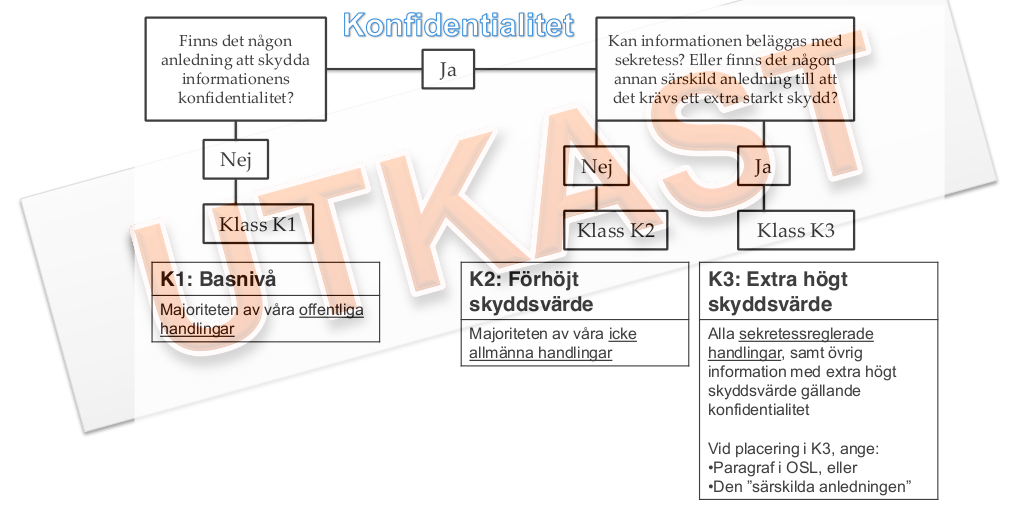
\includegraphics[width=\textwidth]{miun-klassificering.png}
    \caption{Universitetets förslag på klassificeringsmodell för 
    konfidentialitet.}
  \end{figure}
\end{frame}

\subsection{Riskanalys}

\begin{frame}{Riskanalys}
  \begin{itemize}
    \item Används för att anpassa skyddet efter verksamhetens tillgångar.
    \item Genererar en förteckning över
      \begin{itemize}
        \item befintliga hot,
        \item hotens skadeverkningar, och
        \item förslag på riskhantering.
      \end{itemize}
  \end{itemize}
\end{frame}

\begin{frame}{Riskmatris}
  \begin{figure}
    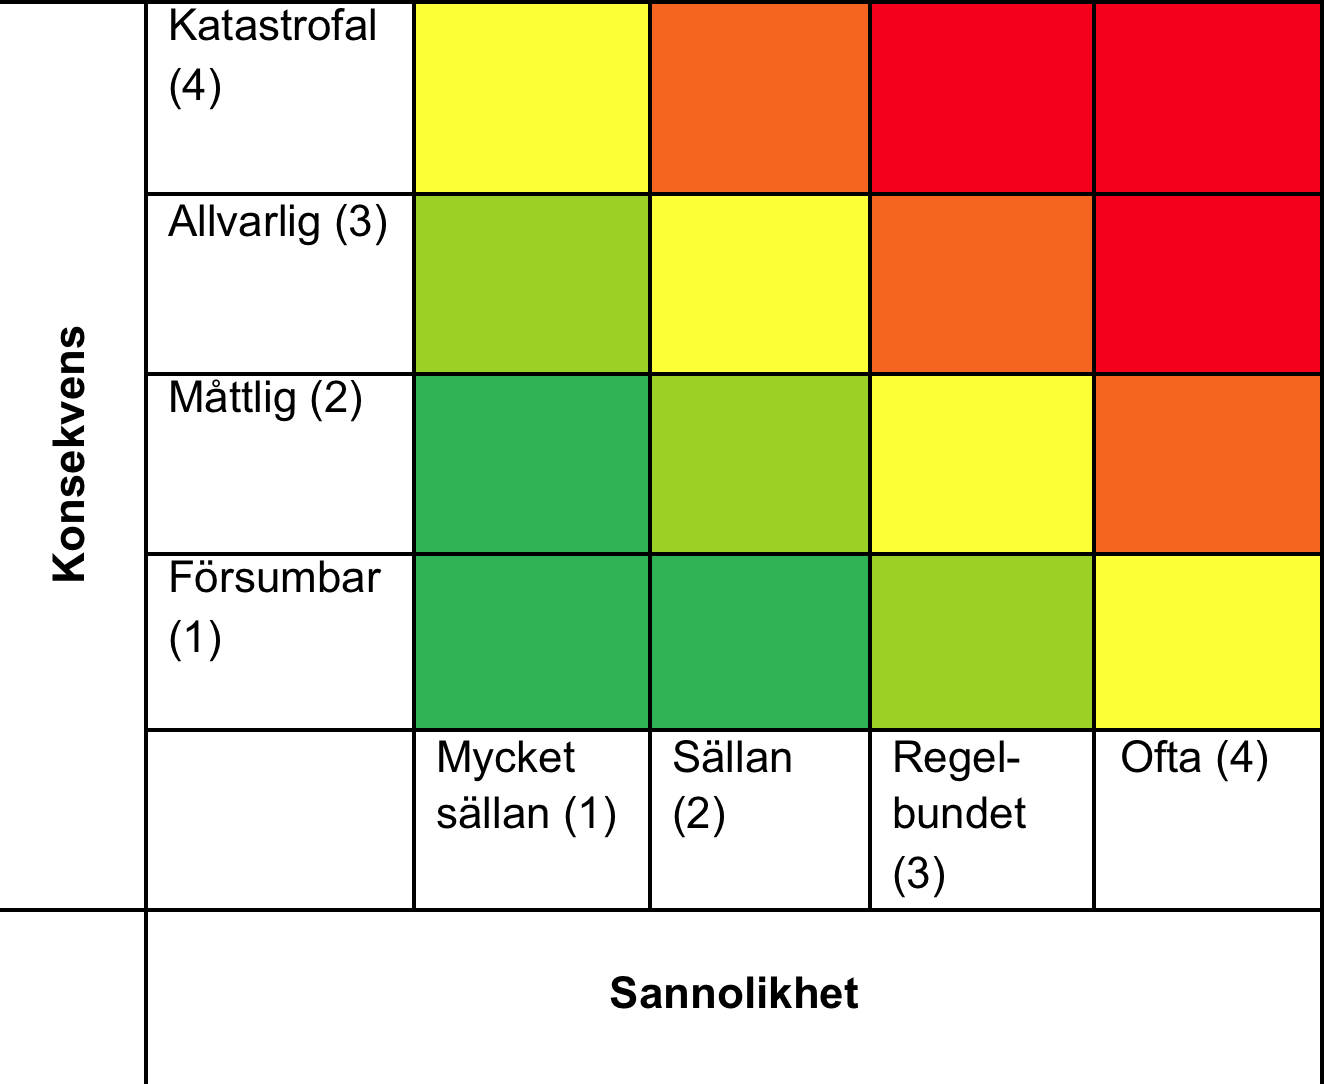
\includegraphics[height=0.7\textheight]{riskmatris.png}
    \caption{En riskmatris.}
  \end{figure}
\end{frame}

\begin{frame}{Formella metoder?}
  \begin{itemize}
    \item Finns forskning som tagit fram mer formella metoder att göra detta.
    \item Bättre då det ger mer objektivitet.
    \item Dock är de svårare att använda.
  \end{itemize}
\end{frame}

\section{Gapanalys}

\subsection{Vad är gapanalys?}

\begin{frame}
  \begin{itemize}
    \item Analysera gapet mellan verksamhetens nuvarande och uppsatta 
      informationssäkerhetsmål.
    \item Metodstödet använder de normer som beskrivs i ISO 27002 istället för 
      verksamhetens mål.
    \item Resultatet visar alltså hur organisationens säkerhet står sig 
      i jämförelse med förväntningarna i ISO 27002.
  \end{itemize}
\end{frame}

\begin{frame}
  Undersöker vilka säkerhetsåtgärder som
  \begin{itemize}
    \item finns och fungerar,
    \item finns men inte fungerar,
    \item inte finns,
    \item inte behövs.
  \end{itemize}
\end{frame}

\begin{frame}{När genomförs gapanalys?}
  \begin{itemize}
    \item Om man vill införa LIS\@.
    \item Om man vill mäta, granska eller verifiera sin 
      informationssäkerhetsnivå.
    \item Om man vill ställa krav på sin informationssäkerhetsnivå.
  \end{itemize}
\end{frame}

\subsection{Hur ska den genomföras?}

\begin{frame}{Krav för gapanalys}
  Analysledaren måste
  \begin{itemize}
    \item känna till verksamhetens behov och krav,
    \item känna till existerande styrdokument för säkerhetsarbetet,
    \item ha god kännedom och förståelse för normerna i standarden.
  \end{itemize}
\end{frame}

\begin{frame}
  \begin{itemize}
    \item Ha ett tydligt beslut att gapanalys ska genomföras,
    \item eller ha mandat att fatta detta beslut.
    \item Använd MSB:s checklista för gapanalys~\cite{MSB2011gb}.
  \end{itemize}
\end{frame}

\subsection{En checklista}

\begin{frame}
  \begin{itemize}
    \item Utgår från ISO 27002.
    \item Innehåller 133 säkerhetsåtgärder.
    \item Varje säkerhetsåtgärd har en eller flera nivåstyrande frågor som 
      ligger till grund för ett betyg mellan 0-3.
    \item Varje säkerhetsåtgärd hör till ett avsnitt.
    \item Varje avsnitt hör till ett kapitel (område).
    \item Totalt finns 11 kapitel.
  \end{itemize}
\end{frame}

\begin{frame}{Checklistan}
  \begin{itemize}
    \item Av totalt 133 säkerhetsåtgärder är 62 (55) kritiska att införa.
    \item De kritiska åtgärderna är en basnivå för informationssäkerheten.
  \end{itemize}
\end{frame}

\subsection{Praktiskt genomförande}

\begin{frame}{Vem?}
  \begin{itemize}
    \item Analysledare.
    \item Experter i verksamheten som är bäst lämpade att svara på respektive 
      område i checklistan.
    \item Behöver inte nödvändigtvis vara chefer.
  \end{itemize}
\end{frame}

\begin{frame}{Praktiskt genomförande}
  \begin{itemize}
    \item Boka in möte med områdesexperterna som ska besvara frågorna.
    \item Skicka ut relevanta frågor till experterna.
    \item Vid mötet: gå igenom frågorna från början till slut.
    \item Börja med nivåstyrande frågorna.
  \end{itemize}
\end{frame}

\begin{frame}{Nivåstyrande frågor}
  \begin{figure}
    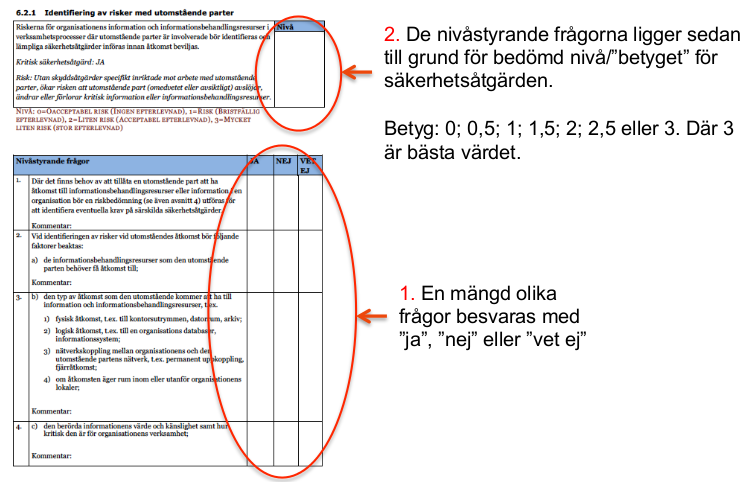
\includegraphics[height=0.7\textheight]{gap-nivafragor.png}
    \caption{Nivåstyrande frågor som ger bedömt värde på säkerhetsåtgärd.}
  \end{figure}
\end{frame}

\begin{frame}{Sammanställning av delavsnitt}
  \begin{figure}
    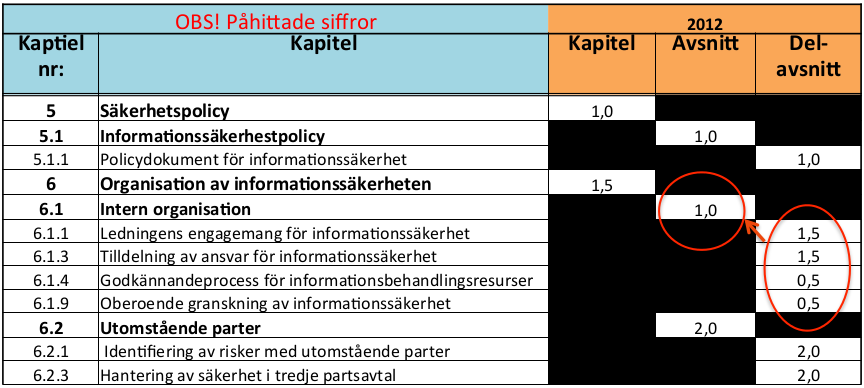
\includegraphics[width=\textwidth]{gap-sammanstallning.png}
    \caption{Betygen för delavsnitt ger betyg för avsnitt.}
  \end{figure}
\end{frame}

\begin{frame}{Sammanställning av avsnitt}
  \begin{figure}
    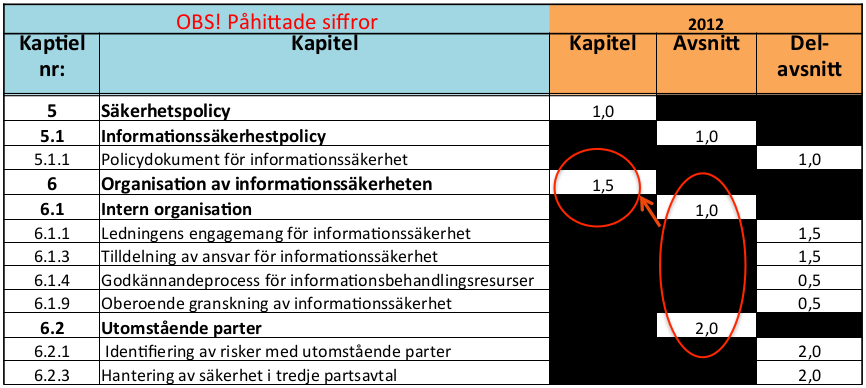
\includegraphics[width=\textwidth]{gap-kapitel.png}
    \caption{Betygen för avsnitt ger betyg för kapitel.}
  \end{figure}
\end{frame}

\begin{frame}{Sammanställning av betyg}
  \begin{figure}
    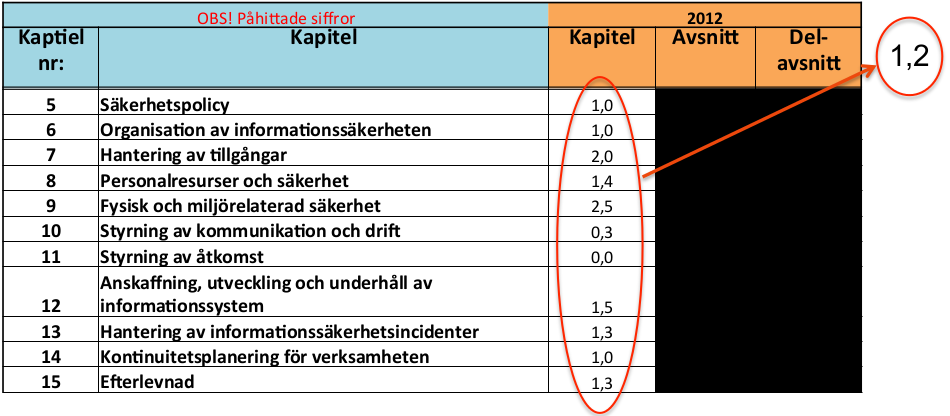
\includegraphics[width=\textwidth]{gap-betyg.png}
    \caption{Betygen för kapitlen ger ett totalbetyg.}
  \end{figure}
\end{frame}

\subsection{Översikt av ISO 27002}

\begin{frame}{ISO 27002}
  \begin{enumerate}
    \item Säkerhetspolicy
    \item Organisation av informationssäkerheten
    \item Hantering av tillgångar
    \item Personalresurser och säkerhet
    \item Fysisk och miljörelaterad säkerhet
    \item Styrning av kommunikation och drift
    \item Styrning av åtkomst
    \item Anskaffning, utveckling och underhåll av informationssystem
    \item Hantering av informationssäkerhetsincidenter
    \item Kontinuitetsplanering för verksamheten
    \item Efterlevnad
  \end{enumerate}
\end{frame}

\begin{frame}{ISO 27002}{Säkerhetspolicy}
  \begin{itemize}
    \item Ange en viljeriktning för verksamhetens informationssäkerhetsarbete.
    \item Arbetet som genomförs måste uppfylla lagkrav och förväntningar.
    \item Har en kritisk säkerhetsåtgärd: policydokument för infosäk.
  \end{itemize}
\end{frame}

\begin{frame}{ISO 27002}{Organisation av informationssäkerheten}
  \begin{itemize}
    \item Ska finnas ett ramverk inom organisationen som styr 
      informationssäkerhetsarbetet.
    \item Styrdokument ska vara beslutade.
    \item Det ska finnas ansvarsfördelning.
    \item Innehåller sex kritiska säkerhetsåtgärder.
  \end{itemize}
\end{frame}

\begin{frame}{ISO 27002}{Hantering av tillgångar}
  \begin{itemize}
    \item Organisationens tillgångar ska få ett lämpligt skydd.
    \item Har två kritiska säkerhetsåtgärder: förteckning av tillgångar, 
      riktlinjer för klassificering.
  \end{itemize}
\end{frame}

\begin{frame}{ISO 27002}{Personalresurser och säkerhet}
  \begin{itemize}
    \item Ska ta informationssäkerheten i beaktande innan, under och efter 
      anställning i organisationen.
    \item Bakgrundskontroller, internutbildning, avsluta behörigheter efter 
      anställning.
    \item Har tre kritiska säkerhetsåtgärder.
  \end{itemize}
\end{frame}

\begin{frame}{ISO 27002}{Fysisk och miljörelaterad säkerhet}
  \begin{itemize}
    \item Förhindra obehörigt tillträde.
    \item Minska risken för skador på informationstillgångar.
    \item Har fyra kritiska säkerhetsåtgärder.
  \end{itemize}
\end{frame}

\begin{frame}{ISO 27002}{Styrning av kommunikation och drift}
  \begin{itemize}
    \item Informationsbehandlingsresurser ska ha en säker drift.
    \item Tydlig ansvarsfördelning och dokumentation för detta.
    \item Har 14 kritiska säkerhetsåtgärder.
  \end{itemize}
\end{frame}

\begin{frame}{ISO 27002}{Styrning av åtkomst}
  \begin{itemize}
    \item Åtkomst till system bör styras utifrån verksamhets- och 
      säkerhetskrav.
    \item Har tio kritiska säkerhetsåtgärder.
  \end{itemize}
\end{frame}

\begin{frame}{ISO 27002}{Anskaffning, utveckling och underhåll av 
  informationssystem}
  \begin{itemize}
    \item Säkerställa att nya och befintliga informationssystem håller god 
      säkerhetsnivå.
    \item Har sju kritiska säkerhetsåtgärder.
  \end{itemize}
\end{frame}

\begin{frame}{ISO 27002}{Hantering av informationssäkerhetsincidenter}
  \begin{itemize}
    \item Inträffade incidenter ska tas om hand.
    \item Minska risken för att incidenten sker igen.
    \item Har två kritiska säkerhetsåtgärder.
  \end{itemize}
\end{frame}

\begin{frame}{ISO 27002}{Kontinuitetsplanering för verksamheten}
  \begin{itemize}
    \item Motverka avbrott i verksamheten.
    \item Lära sig hantera avbrott som ändå uppstår.
    \item Har tre kritiska säkerhetsåtgärder.
  \end{itemize}
\end{frame}

\begin{frame}{ISO 27002}{Efterlevnad}
  \begin{itemize}
    \item Organisationen ska efterleva de externa och interna krav som finns på 
      informationssäkerhetsarbetet.
    \item Har tre kritiska säkerhetsåtgärder.
  \end{itemize}
\end{frame}

\subsection{Resultat}

\begin{frame}{Resultat av gapanalys}
  \begin{itemize}
    \item Vilket skydd är infört?
    \item Vilken omfattning och kvalitet finns på det införda skyddet?
    \item Vilka svagheter och styrkor som finns i det införda skyddet?
    \item Hur kan man gå vidare med att implementera LIS\@?
  \end{itemize}
\end{frame}

\begin{frame}{Slutrapport}
  \begin{itemize}
    \item Hur är arbetet genomfört?
    \item Vilka ingångsvärden är använda?
    \item Resultatet av analysen.
    \item Sammanfattning av resultatet.
    \item Förslag på vidare arbete.
  \end{itemize}
\end{frame}


\section{Utforma}

\subsection{Åtgärder}

\begin{frame}{Att välja säkerhetsåtgärder}
  \begin{figure}
    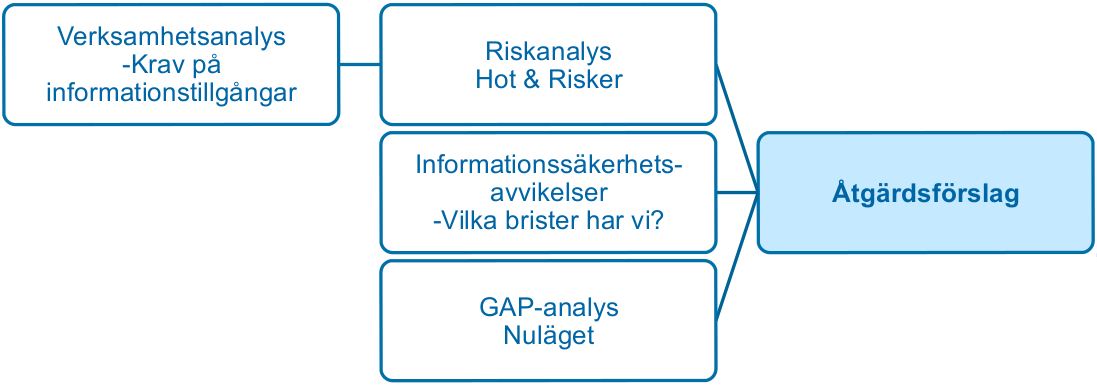
\includegraphics[width=\textwidth]{msb-atgarder.png}
    \caption{Att välja säkerhetsåtgärder.}
  \end{figure}
\end{frame}

\begin{frame}{Att välja säkerhetsåtgärder}
  \begin{description}
    \item[Best practice] Utgår från olika säkerhetsåtgärder i ISO 27002.
    \item[Riskanalys] Skräddarsyr säkerhetsåtgärder efter behov utan 
      utgångspunkt i någon norm.
  \end{description}
  \begin{itemize}
    \item Grundläggande analyser -- behovet av skydd.
    \item Kommer skyddet att ge effekt?
    \item Fokus på \emph{om} de ska införas, inte \emph{hur}.
  \end{itemize}
\end{frame}
\begin{frame}{Typer av åtgärder}
  \begin{itemize}
    \item Styrdokument.
    \item Analyser, övervakning.
    \item Tekniskt skydd.
    \item Utbildningar.
    \item Processer.
  \end{itemize}
\end{frame}

\subsection{Processer}
\begin{frame}{Utforma säkerhetsprocesser}
  \begin{itemize}
    \item Sammanhörande aktiviteter som svarar mot ett definierat behov.
    \item Integrera gärna med befintliga processer.
    \item Exempelvis LIS (strategisk nivå).
    \item Exempelvis informationssäkerhetsklassificering, åtkomsthantering 
      (operativ nivå).
  \end{itemize}
\end{frame}
\begin{frame}{Utforma processer}
  \begin{itemize}
    \item Behöver bred kompetens.
    \item Representera hela organisationen.
    \item Underlättar att samordna med befintliga processer.
  \end{itemize}
\end{frame}

\subsection{Styrdokument}
\begin{frame}{Utforma styrdokument}
  \begin{itemize}
    \item Börja med en policy, organisationens viljeriktning.
    \item Identifiera befintliga dokument: revidera, upphäva, införa nya.
    \item Anpassa efter nuvarande dokumentstruktur.
  \end{itemize}
\end{frame}
\begin{frame}{Utforma styrdokument}
  Glöm inte
  \begin{itemize}
    \item versionshantering,
    \item dokumentägare,
    \item beslutsdatum,
    \item beslutare.
  \end{itemize}
  Skriv dem för att läsas.
\end{frame}


\section{Införa}
\begin{frame}{Införa}
  \begin{itemize}
    \item Säkerhetsprocesser är utformade och beslut finns för 
      säkerhetsåtgärder.
    \item Kan göras i projekt eller i linjeorganisationen.
  \end{itemize}
\end{frame}

\subsection{Planera genomförande}
\begin{frame}{Planera genomförande}
  \begin{itemize}
    \item Finns något leveransobjekt som bör prioriteras?
      (Strategisk vinning?)
    \item Är vissa leveransobjekt beroende av varandra?
    \item Vad kan konstrueras, vad kan anskaffas?
    \item Behöver tidsplan och kommunicera arbetet.
  \end{itemize}
\end{frame}

\subsection{Konstruera och anskaffa}
\begin{frame}{Konstruera och anskaffa}
  \begin{description}
    \item[Konstruera] Organisationen utvecklar själv.
    \item[Anskaffa] Organisationen köper leveransobjekt utifrån.
  \end{description}
  \begin{figure}
    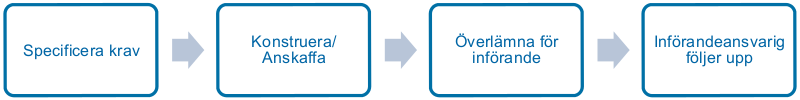
\includegraphics[width=\textwidth]{infora.png}
    \caption{Process för att konstruera och anskaffa.}
  \end{figure}
\end{frame}
\begin{frame}{Kravställning}
  \begin{itemize}
    \item Viktigt med tydlig kravställning.
    \item IT-avdelningen vet inte hur skyddsvärd information den hanterar -- 
      måste specificera!
    \item Tänk på användbarheten för att få organisationen att inte gå runt 
      åtgärderna.
  \end{itemize}
\end{frame}

\subsection{Inför}
\begin{frame}{Inför}
  \begin{itemize}
    \item En samordnare, kallad införandeledare.
    \item Flera införandeansvariga: ansvariga för det praktiska arbetet.
    \item Arbetet genomförs av införandegrupper: chefer för områden berörda av 
      säkerhetsåtgärd.
  \end{itemize}
\end{frame}
\begin{frame}{Införandegrupp}
  Fokusera på:
  \begin{itemize}
    \item Bred representation av verksamheten
    \item Utbilda personal?
      Måste kunna använda säkerhetsåtgärderna.
    \item Vem ska förvalta och hur?
      Behöver förvaltningsplan.
    \item Ska göra organisationen mottaglig för åtgärderna.
  \end{itemize}
\end{frame}
\begin{frame}{Förändra beteende}
  \begin{itemize}
    \item Många säkerhetsåtgärder kräver förändrat beteende.
    \item Kommunicera och förklara \emph{varför} -- målgruppsanpassa detta!
  \end{itemize}
\end{frame}


\section{Följa upp}

\subsection{Övervaka}
\begin{frame}{Övervaka}
  \begin{itemize}
    \item Sker löpande på olika nivåer i verksamheten.
    \item Kommer att ligga till grund för en djupare granskning och redovisning 
      för ledningen.
  \end{itemize}
\end{frame}
\begin{frame}{Övervaka}
  Skapa förutsättningar att utvärdera:
  \begin{itemize}
    \item Verkan av LIS\@: tillräckligt skydd mot aktuella hot?
    \item Verkan av säkerhetsåtgärder: har säkerhetsåtgärderna införts?
    \item Påverkan på informationstillgångar: har sekretessen blivit bättre?
  \end{itemize}
\end{frame}
\begin{frame}{Incidenthantering}
  \begin{itemize}
    \item En del av övervakningen som syftar till att upptäcka nya hot.
    \item Upptäcka brister i åtgärder för tidigare kända hot.
    \item Innefattar även att åtgärda dessa brister.
  \end{itemize}
  \begin{figure}
    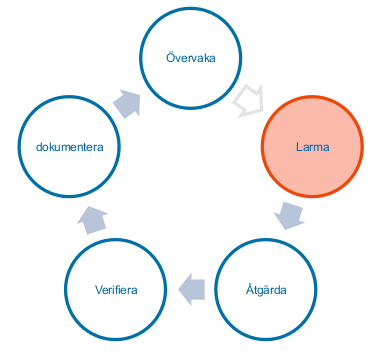
\includegraphics[height=0.4\textheight]{overvakning.png}
    \caption{Cykel för övervakning och incidenthantering.}
  \end{figure}
\end{frame}

\subsection{Granska}
\begin{frame}{Granska}
  \begin{itemize}
    \item En djupare analys av övervakningen.
    \item Del av verksamhetsuppföljning, exempelvis internrevision.
    \item Utgå från information från övervakningen.
    \item Fungerar LIS\@?
  \end{itemize}
\end{frame}
\begin{frame}{Krav på granskning}
  \begin{itemize}
    \item ISO 27001: ledningen ska se till att detta görs -- och ta del av 
      resultatet.
    \item Hur?
      \begin{itemize}
        \item Använd ISO 27001 för LIS\@.
        \item Använd ISO 27002 för säkerhetsåtgärderna.
      \end{itemize}
    \item Vem?
      Oberoende part (revisor) med stöd av LIS-ansvarig.
  \end{itemize}
\end{frame}

\subsection{Ledningens genomgång}
\begin{frame}{Ledningens genomgång}
  \begin{itemize}
    \item Ledningen har ansvaret för verksamheten.
    \item Viktigt att de ges möjlighet att förstå resultaten av granskningen.
    \item Bra med en årlig genomgång av informationssäkerheten.
  \end{itemize}
\end{frame}
\begin{frame}{Ledningens genomgång}
  \begin{itemize}
    \item Genomförs av informationssäkerhetsansvarig och experterna från 
      gapanalysen.
    \item Bör göras en gång per år när det är lämpligt utefter övriga 
      verksamheten.
  \end{itemize}
\end{frame}
\begin{frame}{\insertsubsectionhead}
  \begin{itemize}
    \item Ska innefatta resultat av granskningar, sårbarheter och hot som inte 
      behandlats tillräckligt väl vid senaste riskbedömningen, \dots
    \item Ska resultera i beslut som rör förbättring av verkan av LIS, 
      uppdatering av riskbedömnings- och riskbehandlingsplanen, \dots
  \end{itemize}
\end{frame}


\section{Förbättra}

\subsection{Utveckla LIS och skyddet}
\begin{frame}{\insertsubsectionhead}
  \begin{itemize}
    \item Använd resultat av uppföljningar och ledningens genomgång.
    \item Kravs strukturerat arbetssätt -- PDCA-cykeln.
    \item Standardisera: inför åtgärder i styrdokument, se till att de införs 
      korrekt.
      \begin{itemize}
        \item \enquote{Men så här har vi ju alltid gjort!}
      \end{itemize}
  \end{itemize}
\end{frame}

\subsection{Kommunicera förbättringar}
\begin{frame}{\insertsubsectionhead}
  Skapa intresse som gör att
  \begin{itemize}
    \item medarbetare \emph{lär sig},
    \item får en \emph{positiv} attityd mot säkerhetsarbetet,
    \item har en \emph{intention} om att arbeta för att öka 
      informationssäkerheten,
    \item och med rätt förutsättningar förändrar sitt \emph{beteende}.
  \end{itemize}
\end{frame}
\begin{frame}{\insertsubsectionhead}{''Vi arbetar inte med säkerhet''}
  \begin{quote}
    Vi har inget att skydda, vi har ju inget hemligt.
  \end{quote}
  \begin{quote}
    Det är skillnad på dem som bara jobbar med säkerhet, och mig som faktiskt 
    har ett jobb att sköta.
  \end{quote}
  \begin{quote}
    Det händer ju aldrig oss \dots de här åtgärderna behövs inte.
  \end{quote}
  \begin{quote}
    Det kostar för mycket med säkerhet, är det verkligen värt pengarna?
  \end{quote}
\end{frame}



%%%%%%%%%%%%%%%%%%%%%%

\begin{frame}[allowframebreaks]{Referenser}
	\small
  \printbibliography{}
\end{frame}

\end{document}

